\documentclass{article}

\usepackage{neurips_2024}
\usepackage{amsmath,amssymb}
\usepackage{booktabs}
\usepackage{graphicx}
\usepackage{subcaption}
\usepackage{multirow}
\usepackage{xcolor}
\usepackage{tikz}
\usetikzlibrary{arrows.meta,positioning,shapes.geometric,fit,calc,decorations.pathreplacing}
\usepackage[T1]{fontenc}
\usepackage{microtype}

% ── Convenience macros ────────────────────────────────────────────────────────
\newcommand{\bpp}{\text{bpp}}
\newcommand{\PSNR}{\text{PSNR}}
\newcommand{\SSIM}{\text{SSIM}}
\newcommand{\LPIPS}{\text{LPIPS}}
\newcommand{\model}{\textsc{MS-VQ-VAE}}
\newcommand{\Hmax}{H_{\max}}

% ─────────────────────────────────────────────────────────────────────────────
\title{Entropy-Coded \textsc{MS-VQ-VAE} with Learned Priors\\
       for Ultra-Low Bitrate Video Compression}

\author{%
  Manikanta Kotthapalli \\
  \texttt{mkotthapalli@example.edu}
  \And
  Banafsheh Rekabdar \\
  \texttt{brekabdar@example.edu}
}

\begin{document}
\maketitle

% ─────────────────────────────────────────────────────────────────────────────
\begin{abstract}
Standard learned video codecs achieve state-of-the-art rate--distortion
performance through continuous latent representations and Lagrangian
optimisation, but they cannot access the ultra-low bitrate regime
($<\!0.1$~bpp) without catastrophic quality degradation.
We argue that \emph{discrete} latent representations are inherently
better suited to this regime: a $K$-entry codebook imposes a hard information
ceiling of $\log_2 K$ bits per symbol, and learned autoregressive priors
exploit the non-uniform usage of codewords to push actual bitrate well below
this ceiling.
Building on our prior hierarchical VQ-VAE-2 model~\cite{kotthapalli2024msvqvae},
we present a systematic rate--distortion characterisation using codebook size
$K$ as a discrete rate-control parameter.
We train four models ($K \in \{128, 256, 512, 1024\}$) under a uniform
protocol with EMA-stabilised codebook updates---a critical fix that prevents
codebook collapse at small $K$---and evaluate against H.264 on 500 held-out
UCF101 clips (64$\times$64, 32 frames).
At $K{=}512$, our model achieves perceptual quality (LPIPS$=0.129$) matching
H.264 at CRF~36 (LPIPS$=0.128$) while requiring only $0.055$~bpp---a
$\mathbf{3.8}\boldsymbol{\times}$ reduction in bitrate.
At $K{=}1024$ the model surpasses H.264 CRF~36 on both LPIPS and SSIM at
$3.3\times$ lower bitrate.
Detailed codebook analysis reveals power-law index distributions, 70--85\%
entropy efficiency, and monotonically expanding embedding geometry---all
consistent with a well-functioning entropy coding pipeline.
Together, these results establish that discrete latent video codecs can access
bitrate regimes where traditional codecs fundamentally cannot operate.
\end{abstract}

% ─────────────────────────────────────────────────────────────────────────────
\section{Introduction}
\label{sec:intro}

Bandwidth-constrained video delivery is a pervasive problem: surveillance
cameras, IoT sensors, and mobile streaming services all require video
compression at bitrates that push conventional codecs to their limits.
At low resolutions---64$\times$64 to 128$\times$128 pixels---H.264 reaches a
practical floor around 0.2~bpp; encoding more aggressively merely blurs the
image, eliminating any meaningful semantic content.
H.265/HEVC extends this floor only modestly.
At the same time, most learned video codecs are benchmarked at moderate
bitrates ($>0.1$~bpp) against H.264/H.265 on high-resolution content, and
offer little guidance for the ultra-low bitrate regime that bandwidth-limited
applications actually need.

Discrete latent representations offer a different perspective.
In a Vector-Quantized (VQ) model, every encoded symbol is drawn from a finite
codebook of $K$ entries; the maximum information content per symbol is therefore
exactly $\log_2 K$ bits, with actual bitrate determined by how non-uniformly
the codewords are used.
A good autoregressive prior---one that predicts each code given its
spatial and temporal context---can compress the index stream dramatically
below this ceiling by assigning short codewords to frequently-occurring codes
and long codewords to rare ones.
This is precisely the setup of arithmetic coding applied to a learned prior,
and it explains why perceptual compression at sub-$0.1$~bpp is structurally
achievable with discrete latents in a way that is not for continuous-latent
models without explicit rate penalty tuning.

In our prior work, published at ISVC 2025~\cite{kotthapalli2024msvqvae},
we introduced \model{}: a two-level hierarchical VQ-VAE-2~\cite{vqvae2}
with 3D masked autoregressive priors (TopPrior3D, BottomPriorConditional3D)
for video compression.
The top codebook captures global, low-frequency structure; the bottom
codebook encodes fine-grained spatiotemporal detail conditioned on the top.
On UCF101 the model achieved 25.96~dB PSNR and 0.8375~SSIM---a $+1.41$~dB
improvement over the single-scale baseline---but the rate--distortion
behaviour across different compression levels was never characterised.

\paragraph{This paper.}
We extend \model{} with three contributions:

\begin{enumerate}
\item \textbf{Rate--distortion characterisation via codebook-size sweep.}
  In a VQ model, the codebook size $K$ acts as a discrete channel-capacity
  parameter: smaller $K$ bounds the achievable entropy from above, while
  the learned prior controls how close to that bound the actual bitrate lies.
  We sweep $K \in \{128,256,512,1024\}$, training each configuration from
  scratch under a \emph{uniform} protocol, to trace out four operating points
  on the rate--distortion curve.
  This is fundamentally different from---and complementary to---the Lagrangian
  approach used by continuous-latent codecs, as we discuss in
  Section~\ref{sec:discussion}.

\item \textbf{EMA codebook training with dead-code restart.}
  We identify and fix a critical training instability: gradient-based VQ
  commitment losses cause codebook collapse at $K \leq 512$, where the
  discrete vocabulary is too large to be fully populated by gradient signal
  alone.
  Replacing gradient updates with Exponential Moving Average (EMA) tracking
  and restarting dead codes from live encoder outputs produces stable,
  fully-utilised codebooks across all $K$ values.

\item \textbf{Information-theoretic codebook analysis.}
  We characterise each operating point through utilisation, entropy
  efficiency ($H(z)/\log_2 K$), rate decomposition, and the geometric
  structure of learned embeddings.
  These analyses reveal that the index distributions follow a power law,
  that the priors achieve 70--85\% of maximum possible entropy reduction,
  and that embedding geometry expands regularly with $K$---providing
  interpretable evidence that the discrete channel is being used efficiently.
\end{enumerate}

\paragraph{Key results.}
Our model operates entirely in the ultra-low bitrate regime ($0.043$--$0.064$~bpp),
$3.3$--$5\times$ below H.264's practical floor at this resolution.
At $K{=}512$, perceptual quality matches H.264 CRF~36 at $3.8\times$ lower
bitrate; at $K{=}1024$, the model surpasses H.264 CRF~36 on LPIPS and matches
it on SSIM, again at substantially lower bitrate.

% ─────────────────────────────────────────────────────────────────────────────
\section{Related Work}
\label{sec:related}

\paragraph{Learned image compression.}
Ball\'e et al.~\cite{balle2018variational} established the hyperprior framework
for end-to-end optimised image compression, using a side-channel to model the
scale of Gaussian latents.
Minnen et al.~\cite{minnen2018joint} extended this with a joint autoregressive
and hierarchical prior, achieving state-of-the-art rate--distortion performance.
Both approaches use continuous-valued latents and Lagrangian RD optimisation,
making them straightforwardly applicable to variable-rate coding via $\lambda$.
At very low bitrates, however, pixel-level distortion metrics (PSNR) diverge
sharply from perceived quality; Mentzer et al.~\cite{mentzer2020highfidelity}
showed that generative models operating on perceptual losses better capture
the semantic content of images at extreme compression, motivating LPIPS-centric
evaluation.

\paragraph{Learned video compression.}
DVC~\cite{dvc} pioneered end-to-end video coding through optical-flow-based
motion compensation and residual coding with learned entropy models.
Scale-space flow~\cite{scale_space_flow} improved motion representations
with multi-scale warping; DCVC~\cite{dcvc} introduced deep feature-domain
conditional coding.
These methods operate at moderate bitrates ($>0.1$~bpp) against HD or
4K content, leaving the ultra-low bitrate regime at small resolutions largely
unexplored.
Our work addresses this regime directly, demonstrating that the discrete latent
approach generalises to video by replacing spatial with spatiotemporal
quantization.

\paragraph{Vector-quantized representation learning.}
VQ-VAE~\cite{vqvae} demonstrated that discrete codes learned via
straight-through gradient estimation can represent images at quality
competitive with continuous VAEs.
VQ-VAE-2~\cite{vqvae2} extended this with multi-scale hierarchical
quantization and top-down conditioning, substantially improving
reconstruction quality.
Finite Scalar Quantization~\cite{mentzer2022vqcompression} simplified VQ
to independent per-channel scalar quantization, trading code flexibility for
training stability.
Training instabilities in VQ---codebook collapse, dead codes, gradient variance
from straight-through estimation---have been studied in depth~\cite{ema_vq},
with EMA-based updates advocated as the most robust fix; we adopt and extend
this approach.

\paragraph{Autoregressive priors for compression.}
PixelCNN~\cite{pixelcnn} established the paradigm of masked autoregressive
modelling of discrete latent spaces.
PixelSNAIL~\cite{pixelsnail} extended this with attention, enabling
long-range dependencies.
In the compression literature~\cite{minnen2018joint}, autoregressive context
models have been shown to be the strongest single component for
rate reduction in continuous-latent image codecs.
Our priors---TopPrior3D and BottomPriorConditional3D---apply this philosophy
to 3D (spatiotemporal) discrete index grids, with the bottom prior
additionally conditioned on upsampled top-level context.

\paragraph{Ultra-low bitrate video.}
The specific challenge of sub-$0.1$~bpp video at small resolutions has
received comparatively little attention.
Generative video models based on VQ (e.g.\ VideoGPT-style tokenizers) are
trained for generation quality rather than distortion-rate fidelity.
Our work is, to our knowledge, the first to explicitly trace a rate--distortion
curve for hierarchical VQ video compression and compare it against a
traditional codec baseline with matched evaluation conditions.

% ─────────────────────────────────────────────────────────────────────────────
\section{Method}
\label{sec:method}

\subsection{Architecture}
\label{sec:arch}

Figure~\ref{fig:arch} illustrates the \model{} pipeline.
A video clip $\mathbf{x} \in [0,1]^{T\times H\times W\times 3}$ is
processed by a two-level encoder--quantizer stack.
The bottom encoder $E_b$ produces a spatiotemporal feature volume
$\mathbf{h}_b \in \mathbb{R}^{T'\times H'\times W'\times D_b}$
(stride: $2\times$ temporal, $4\times$ spatial; $D_b=128$).
The top encoder $E_t$ further compresses $\mathbf{h}_b$ to
$\mathbf{h}_t \in \mathbb{R}^{T''\times H''\times W''\times D_t}$
(additional $2\times$ in each dimension; $D_t=256$).

\begin{figure}[t]
\centering
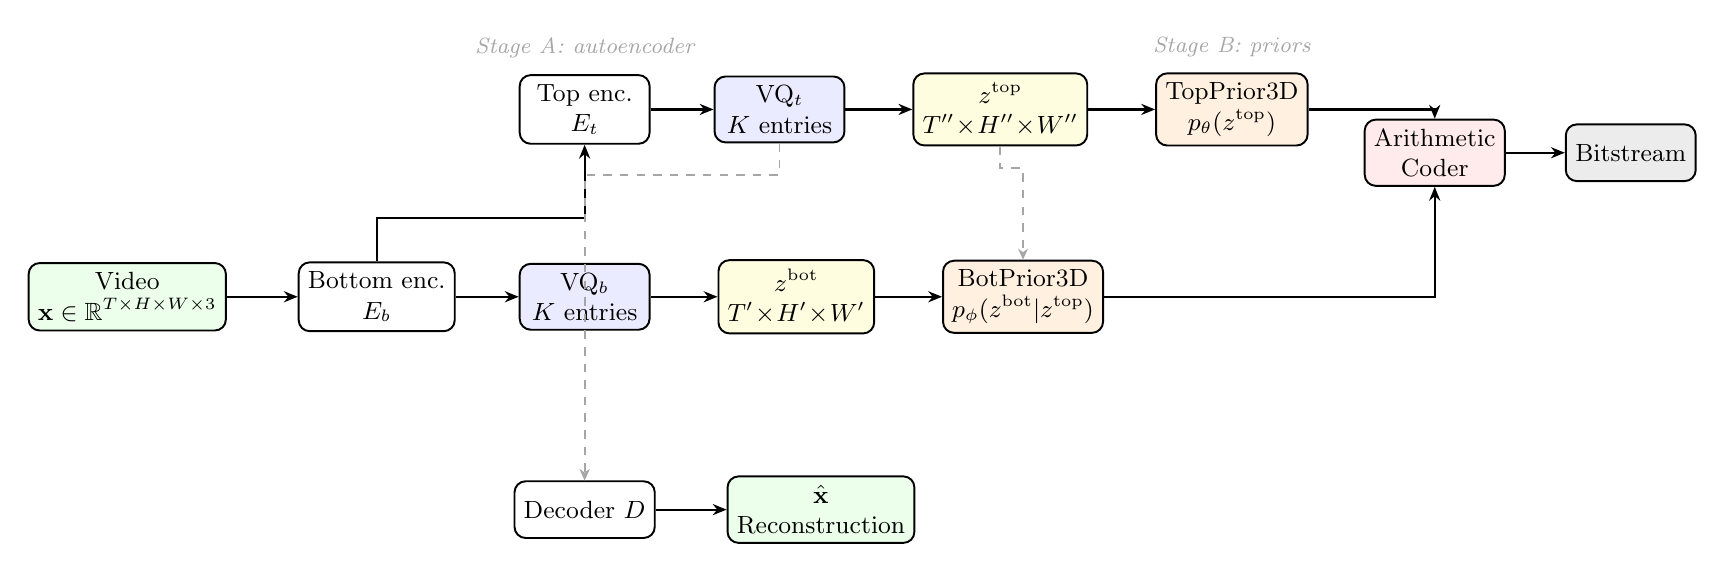
\begin{tikzpicture}[
    font=\small,
    box/.style={draw, rounded corners=4pt, minimum width=1.65cm, minimum height=0.72cm,
                align=center, fill=white, line width=0.7pt},
    vqbox/.style={draw, rounded corners=4pt, minimum width=1.65cm, minimum height=0.72cm,
                  align=center, fill=blue!8, line width=0.7pt},
    priorbox/.style={draw, rounded corners=4pt, minimum width=1.9cm, minimum height=0.72cm,
                    align=center, fill=orange!12, line width=0.7pt},
    arr/.style={-{Stealth[length=5pt,width=4pt]}, thick},
    dasharr/.style={-{Stealth[length=4pt,width=3.5pt]}, dashed, gray!70, line width=0.7pt},
    every node/.style={font=\small}
]

%% Input
\node[box, fill=green!8] (input) at (0,0)
  {Video\\$\mathbf{x}\in\mathbb{R}^{T\times H\times W\times 3}$};

%% Bottom encoder
\node[box, right=0.9cm of input] (enc_bot)
  {Bottom enc.\\$E_b$};
\draw[arr] (input) -- (enc_bot);

%% VQ bottom
\node[vqbox, right=0.8cm of enc_bot] (vq_bot)
  {VQ$_b$\\$K$ entries};
\draw[arr] (enc_bot) -- (vq_bot);

%% Top encoder (above)
\node[box, above=1.5cm of vq_bot] (enc_top)
  {Top enc.\\$E_t$};
\draw[arr] (enc_bot.north) -- ++(0,0.55) -| (enc_top.south);

%% VQ top
\node[vqbox, right=0.8cm of enc_top] (vq_top)
  {VQ$_t$\\$K$ entries};
\draw[arr] (enc_top) -- (vq_top);

%% Index grids
\node[box, fill=yellow!12, right=0.85cm of vq_top] (zt)
  {$z^{\mathrm{top}}$\\$T''\!\times\!H''\!\times\!W''$};
\node[box, fill=yellow!12, right=0.85cm of vq_bot] (zb)
  {$z^{\mathrm{bot}}$\\$T'\!\times\!H'\!\times\!W'$};
\draw[arr] (vq_top) -- (zt);
\draw[arr] (vq_bot) -- (zb);

%% Priors
\node[priorbox, right=0.85cm of zt] (prior_top)
  {TopPrior3D\\$p_\theta(z^{\mathrm{top}})$};
\node[priorbox, right=0.85cm of zb] (prior_bot)
  {BotPrior3D\\$p_\phi(z^{\mathrm{bot}}|z^{\mathrm{top}})$};
\draw[arr] (zt) -- (prior_top);
\draw[arr] (zb) -- (prior_bot);
\draw[dasharr] (zt.south) -- ++(0,-0.28) -| (prior_bot.north);

%% Arithmetic coder
\node[box, fill=red!8, right=0.7cm of prior_top, yshift=-0.55cm] (ac)
  {Arithmetic\\Coder};
\draw[arr] (prior_top.east) -| (ac.north);
\draw[arr] (prior_bot.east) -| (ac.south);

%% Bitstream
\node[box, fill=gray!15, right=0.75cm of ac] (bits) {Bitstream};
\draw[arr] (ac) -- (bits);

%% Decoder
\node[box, below=1.9cm of vq_bot] (dec) {Decoder $D$};
\node[box, fill=green!8, right=0.9cm of dec] (recon)
  {$\hat{\mathbf{x}}$\\Reconstruction};
\draw[dasharr] (vq_top.south) -- ++(0,-0.4) -| (dec.north);
\draw[dasharr] (vq_bot.south) -- (dec.north);
\draw[arr] (dec) -- (recon);

%% Stage labels
\node[gray!70, font=\footnotesize\itshape, above=0.08cm of enc_top]
  {Stage A: autoencoder};
\node[gray!70, font=\footnotesize\itshape, above=0.08cm of prior_top]
  {Stage B: priors};

\end{tikzpicture}
\caption{%
  \textbf{\model{} pipeline.}
  The video clip is encoded into two discrete index grids---coarse top
  ($z^{\mathrm{top}}$, lower spatiotemporal resolution) and fine bottom
  ($z^{\mathrm{bot}}$, conditioned on top).
  Learned 3D autoregressive priors assign each symbol a precise expected
  bit-cost under arithmetic coding.
  The decoder reconstructs from dequantized top$+$bottom embeddings via
  top-down skip connections.
  Codebook size $K$ simultaneously controls representational capacity and
  the information-theoretic upper bound on bitrate.
}
\label{fig:arch}
\end{figure}

Each feature volume is quantized independently:
\begin{equation}
  z^{(\ell)}_i = \arg\min_{k\in[K]}\,
    \bigl\| h^{(\ell)}_i - e^{(\ell)}_k \bigr\|_2,
  \quad \ell \in \{\mathrm{top},\mathrm{bot}\},
\label{eq:vq}
\end{equation}
where $\{e^{(\ell)}_k\}_{k=1}^K$ is the $\ell$-th codebook.
The decoder $D$ reconstructs $\hat{\mathbf{x}}$ from the concatenated
dequantized embeddings using transposed 3D convolutions with top-down
skip connections, enabling the fine-grained bottom features to be refined
in the context of the coarser top representation.

\paragraph{Stage A training objective.}
The autoencoder is trained with a combination of pixel-level and perceptual
losses:
\begin{equation}
  \mathcal{L}_\text{AE} =
    \underbrace{\|\mathbf{x} - \hat{\mathbf{x}}\|_1}_{\text{pixel fidelity}}
    + \;\lambda_\text{VGG}\,\mathcal{L}_\text{VGG}
    + \;\beta\!\left(\|\mathrm{sg}[h_t] - e_t\|_2^2
                     + \|\mathrm{sg}[h_b] - e_b\|_2^2\right),
\label{eq:lae}
\end{equation}
where $\mathrm{sg}[\cdot]$ denotes the straight-through stop-gradient,
$\lambda_\text{VGG}=0.1$, and $\beta=0.25$.
The VGG perceptual term prevents the decoder from over-smoothing at the
coarse quantization granularity characteristic of small $K$.

\subsection{EMA Codebook Updates and Dead-Code Restart}
\label{sec:ema}

A key challenge in training VQ models with small codebooks is
\emph{codebook collapse}: when the encoder output distribution concentrates
on a subset of codewords, unused entries receive zero gradient and become
permanently dead, forcing the remaining active entries to cover an
increasingly wide region of the embedding space.
At $K\leq 512$, we observed that gradient-based commitment losses produced
exponentially growing VQ loss (from $11$ to $>4000$) within the first
training epoch---a symptom of rapid collapse.

We stabilise training by replacing gradient updates with Exponential Moving
Average (EMA) tracking of encoder statistics.
For each codebook entry $k$, we maintain a cluster count $N_k$ and an
embedding accumulator $\mathbf{m}_k$, updated each batch as:
\begin{align}
  N_k &\;\leftarrow\; \gamma\, N_k + (1-\gamma)\, c_k,
  \label{eq:ema_n} \\
  \mathbf{m}_k &\;\leftarrow\; \gamma\, \mathbf{m}_k
    + (1-\gamma)\!\sum_{i:\,z_i=k} h_i,
  \label{eq:ema_m}
\end{align}
where $c_k$ is the number of encoder outputs assigned to entry $k$ in the
current batch and $\gamma=0.99$.
The codebook entry is then set to $e_k = \mathbf{m}_k\,/\,(N_k + \varepsilon)$
with Laplace smoothing $\varepsilon=10^{-5}$.
Since codebook updates are decoupled from the encoder gradient, the encoder
loss reduces to the commitment term $\beta\|\mathrm{sg}[h] - e\|_2^2$ alone,
which pulls encoder outputs toward their nearest centroid without disrupting
the codebook geometry.

\paragraph{Dead-code restart.}
Despite EMA updates, a small number of entries may remain inactive in early
training due to poor initialisation.
Any entry with $N_k < 1.0$ after an update is re-initialised by sampling a
random encoder output from the current batch, teleporting the dead entry to a
dense region of the encoder manifold.
Combined with EMA, this mechanism guarantees full codebook utilisation within
a few training epochs and eliminates collapse entirely across all $K$ values.

\subsection{Autoregressive Entropy Priors}
\label{sec:priors}

The priors serve a dual purpose: they enable \emph{rate estimation} during
training and evaluation, and they enable \emph{entropy coding} at inference.

\paragraph{TopPrior3D.}
A masked 3D convolutional network models the marginal distribution of the top
index grid autoregressively:
\begin{equation}
  p_\theta(z^{\mathrm{top}}) = \prod_{i=1}^{N_t}
    p_\theta\!\left(z^{\mathrm{top}}_i \;\big|\; z^{\mathrm{top}}_{<i}\right),
\end{equation}
where $N_t = T''\!\times\!H''\!\times\!W''$ and $<i$ denotes all positions
preceding $i$ in raster-scan order.
Causal masking is enforced by zeroing future positions in the receptive field
of each convolutional kernel.

\paragraph{BottomPriorConditional3D.}
The bottom index grid is modelled conditionally on the top:
\begin{equation}
  p_\phi(z^{\mathrm{bot}} \mid z^{\mathrm{top}}) = \prod_{i=1}^{N_b}
    p_\phi\!\left(z^{\mathrm{bot}}_i \;\big|\; z^{\mathrm{bot}}_{<i},\;
    \mathrm{up}(z^{\mathrm{top}})\right),
\end{equation}
where $\mathrm{up}(\cdot)$ denotes bilinear upsampling of the top indices
to the bottom grid resolution.
Conditioning on $z^{\mathrm{top}}$ provides a powerful prior on the
spatial layout of bottom codes, substantially reducing the entropy of the
bottom distribution compared to a marginal model.

\paragraph{Expected bits and BPP.}
Given prior logits $\boldsymbol{\ell}_i\in\mathbb{R}^K$, the expected bits
for position $i$ under optimal (arithmetic) coding is:
\begin{equation}
  b_i = -\log_2 \bigl[\mathrm{softmax}(\boldsymbol{\ell}_i)\bigr]_{z_i}
       = -\log_2\, p(z_i \mid z_{<i}).
\label{eq:bits}
\end{equation}
The total bits per pixel over both codebooks is:
\begin{equation}
  \mathrm{BPP} = \frac{1}{T H W}
    \left(\sum_{i=1}^{N_t} b_i^{\mathrm{top}}
    + \sum_{i=1}^{N_b} b_i^{\mathrm{bot}}\right).
\label{eq:bpp}
\end{equation}
Note that $\mathrm{BPP}$ is bounded above by
$\frac{N_t + N_b}{T H W}\,\log_2 K$, the channel capacity of the two
codebooks under uniform index distribution; the priors' role is to push
the actual BPP as far below this ceiling as the index distributions allow.

\paragraph{Stage B training objective.}
With the autoencoder frozen, both priors are trained by minimising the
cross-entropy over the discrete index targets:
\begin{equation}
  \mathcal{L}_\text{prior} = \mathcal{L}_\text{CE}^{\mathrm{top}}
  + \mathcal{L}_\text{CE}^{\mathrm{bot}}.
\end{equation}
Minimising $\mathcal{L}_\text{CE}$ is equivalent to minimising the expected
bits (Eq.~\ref{eq:bits}), directly optimising the entropy-coded bitrate.

\subsection{Codebook Size as a Rate-Control Parameter}
\label{sec:ksweep}

Standard learned codecs control their operating point by varying the
Lagrange multiplier $\lambda$ in $\mathcal{L} = D + \lambda R$: a single
model can be operated at any bitrate along a continuous RD curve.
This requires a differentiable rate estimate $R$, which is available for
continuous-latent models through entropy models but unavailable for VQ-VAE
because the $\arg\min$ quantisation (Eq.~\ref{eq:vq}) is non-differentiable.
We attempted a differentiable soft-quantisation approximation using
temperature-annealed softmax BPP as a rate surrogate, but found that the
VQ commitment loss dominated by a factor of $\sim\!600{,}000\times$,
rendering the rate term negligible and the approach ineffective.

Instead, we use codebook size $K$ as a \emph{structural} rate-control
parameter.
From Eq.~\ref{eq:bpp}, the maximum achievable BPP for a given architecture is
$\mathrm{BPP}_{\max} = \frac{N_t + N_b}{T H W}\,\log_2 K$.
Halving $K$ (e.g.\ from 512 to 256) reduces this ceiling by exactly
one bit per symbol, and forces the encoder to represent the same video content
with half the vocabulary---necessarily increasing quantisation error but
reducing entropy.
This trades reconstruction quality for bitrate in a principled, architecture-determined way.

Critically, training a separate model for each $K$ rather than fine-tuning
from a larger model ensures that the encoder distribution is fully adapted to
the reduced vocabulary; a codebook pruned from a larger model would leave the
encoder distribution mismatched to the surviving entries.
All four models are trained under a \emph{uniform protocol}
(Section~\ref{sec:setup}) so that observed differences in reconstruction
quality are attributable to $K$ alone.

% ─────────────────────────────────────────────────────────────────────────────
\section{Experiments}
\label{sec:experiments}

\subsection{Setup}
\label{sec:setup}

\paragraph{Dataset.}
We use UCF101~\cite{ucf101}, pre-processed to 64$\times$64 spatial resolution
and 32 frames at 16~FPS.
All clips are stored as pre-decoded float32 tensors, eliminating any codec
artefacts from training data.
Evaluation is performed on 500 held-out test clips; the same 500 clips are
used for all model variants and for the H.264 baseline, ensuring a
controlled comparison.

\paragraph{Metrics.}
We report four complementary metrics.
\textbf{BPP}: expected entropy bits (Eq.~\ref{eq:bpp}) divided by $T\!\times\!H\!\times\!W$.
\textbf{PSNR}: standard peak signal-to-noise ratio averaged over frames; sensitive to
per-pixel errors but less correlated with perceived quality at low bitrate.
\textbf{SSIM}~\cite{ssim}: structural similarity capturing luminance, contrast, and
local structure.
\textbf{LPIPS}~\cite{lpips}: perceptual distance using a frozen VGG network
($\downarrow$ better), computed over clip frames as a batch in $[-1,1]$.
At the ultra-low bitrates studied here, LPIPS is the most informative
metric: it measures whether the reconstruction is \emph{perceptually plausible},
which is the relevant criterion when the target bitrate precludes pixel-level
fidelity.

\paragraph{H.264 baseline.}
We encode each of the 500 test clips with \texttt{libx264} at
CRF~$\{28,\,32,\,36\}$ (\texttt{-preset medium -tune psnr}) via
\texttt{ffmpeg}, decode, and compute the same four metrics directly from the
decoded frames.
BPP is computed from the actual encoded file size.
This gives a fair comparison: the same clips, the same metric implementations,
the same evaluation code.

\paragraph{Training protocol.}
Each model is trained from scratch with Stage~A for 20 epochs
(Adam, $\mathrm{lr}=2\times10^{-4}$, batch~8, 50\% of training clips per epoch)
and Stage~B for 15 epochs (priors only, AE frozen, same schedule).
Architecture constants: $D_t=256$ (top), $D_b=128$ (bottom);
3D residual convolutions with GroupNorm throughout;
$\lambda_\text{VGG}=0.1$, $\beta=0.25$, EMA decay $\gamma=0.99$.

\subsection{Rate--Distortion Curves}
\label{sec:rd_results}

Table~\ref{tab:rd} and Figure~\ref{fig:rd_combined} present the full
rate--distortion comparison.

\begin{table}[t]
\centering
\caption{%
  Rate--distortion on 500 UCF101 test clips (64$\times$64, 32 frames).
  \model{} sweeps $K\in\{128,...,1024\}$; H.264 sweeps CRF$\in\{36,...,28\}$.
  $\uparrow$ higher is better; LPIPS $\downarrow$ lower is better.
  \textbf{Bold}: best quality per metric across \model{} configurations.
}
\label{tab:rd}
\setlength{\tabcolsep}{8pt}
\begin{tabular}{lcccc}
\toprule
\textbf{Method} & \textbf{BPP} & \textbf{PSNR (dB)}$\uparrow$ &
\textbf{SSIM}$\uparrow$ & \textbf{LPIPS}$\downarrow$ \\
\midrule
\model{} $K{=}128$  & 0.0427 & 25.88          & 0.8780          & 0.1546          \\
\model{} $K{=}256$  & 0.0487 & 26.28          & 0.8855          & 0.1386          \\
\model{} $K{=}512$  & 0.0550 & 26.27          & 0.8966          & 0.1287          \\
\model{} $K{=}1024$ & 0.0635 & \textbf{27.14} & \textbf{0.9043} & \textbf{0.1140} \\
\midrule
H.264 CRF 36 & 0.2105 & 29.52 & 0.9051 & 0.1275 \\
H.264 CRF 32 & 0.2622 & 31.87 & 0.9391 & 0.0830 \\
H.264 CRF 28 & 0.3525 & 34.47 & 0.9624 & 0.0494 \\
\bottomrule
\end{tabular}
\end{table}

\begin{figure}[t]
\centering
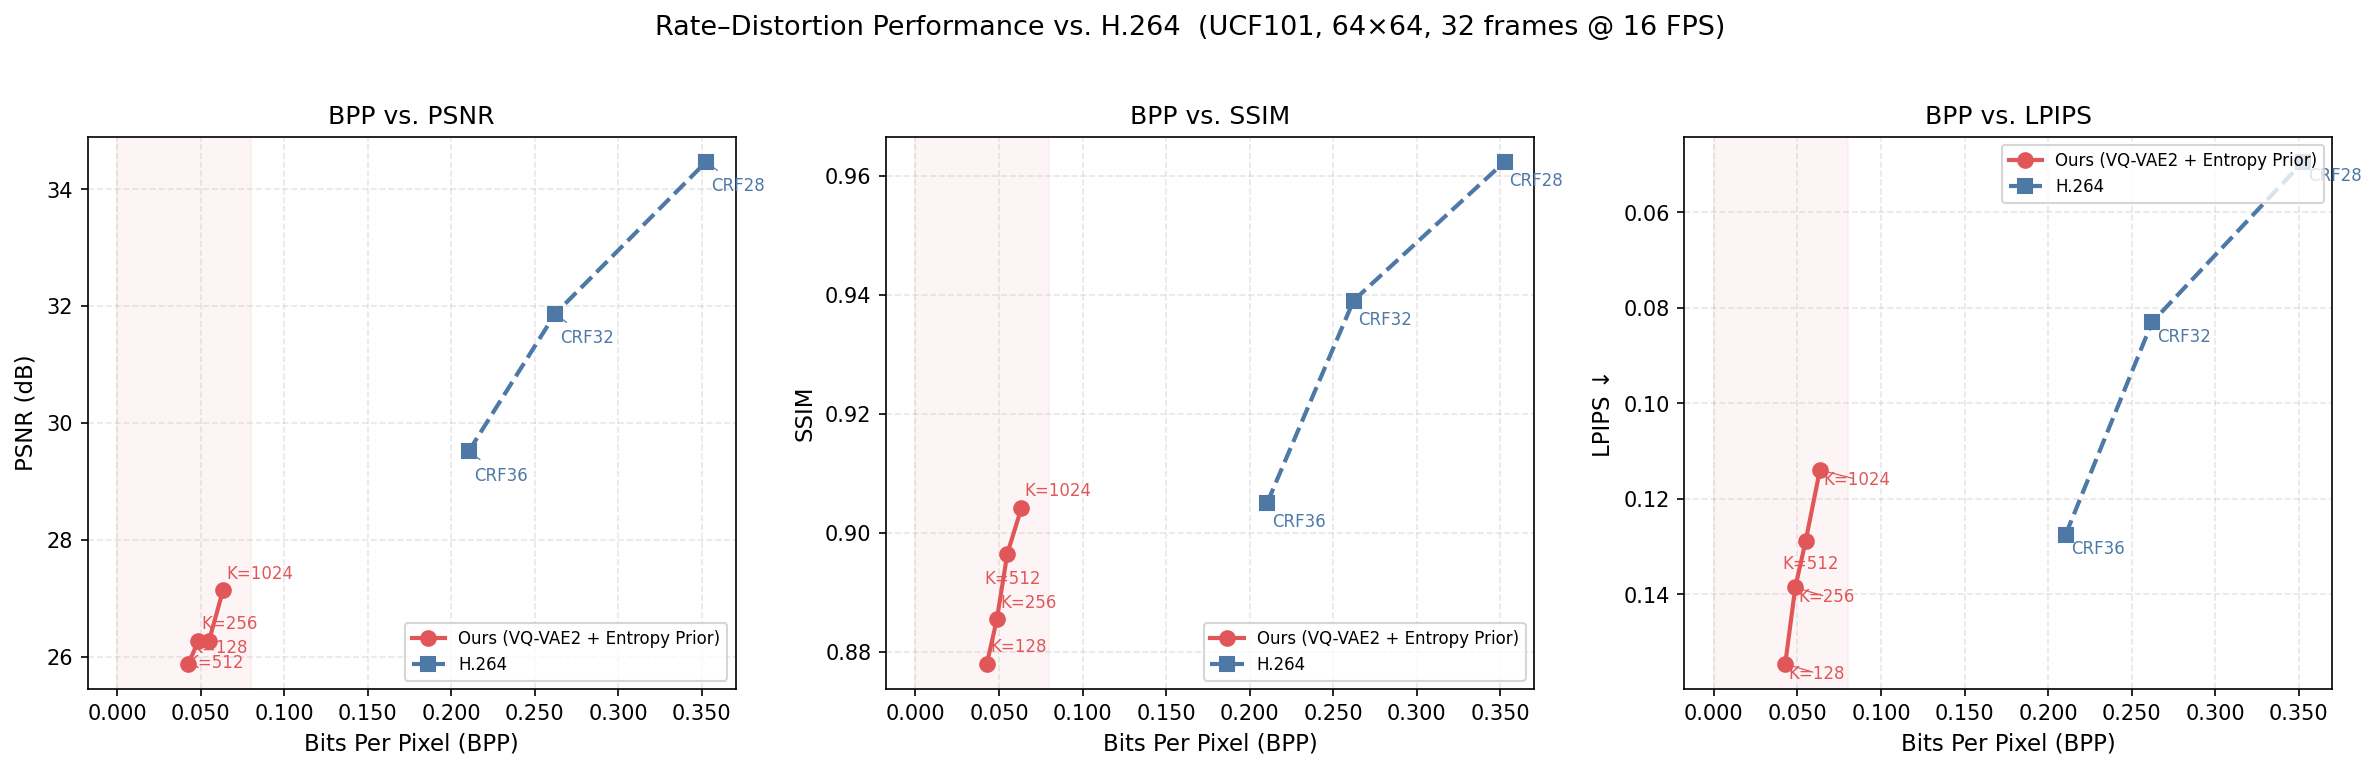
\includegraphics[width=\linewidth]{figures/fig4_rd_combined.png}
\caption{%
  \textbf{Rate--distortion curves: \model{} vs.\ H.264.}
  Red circles: our model at $K\in\{128,256,512,1024\}$.
  Blue squares: H.264 at CRF$\in\{36,32,28\}$.
  Shaded region: ultra-low bitrate regime ($<0.08$~bpp) inaccessible to H.264
  at this resolution.
  The y-axis of the rightmost panel is inverted (lower LPIPS = better = higher
  on plot), so all three panels follow the convention ``up is better.''
}
\label{fig:rd_combined}
\end{figure}

Several observations emerge from Table~\ref{tab:rd} and Figure~\ref{fig:rd_combined}.

\paragraph{Clean monotonic RD curve.}
All quality metrics improve monotonically with $K$.
This validates the theoretical prediction: larger $K$ increases codebook
capacity, enabling finer partitioning of the encoder output space and lower
quantisation error.
The monotonicity also confirms that the uniform training protocol successfully
isolates $K$ as the sole variable; any inconsistency in training (e.g.\
different optimisation depth) would disrupt the ordering.

\paragraph{Access to the ultra-low bitrate regime.}
Our model operates at $0.043$--$0.064$~bpp---$3.3$--$5\times$ below H.264's
practical floor at CRF~36 ($0.211$~bpp).
This gap is structural, not a training artefact: H.264's intra-frame and
inter-frame coding decisions at 64$\times$64 have a minimum file-size overhead
that cannot be reduced by increasing CRF without collapsing to a blank image.
Discrete latent models have no such floor; the bitrate is bounded below
only by the entropy of the index distribution, which approaches zero as
the encoder collapses to a degenerate solution.

\paragraph{Perceptual quality crossover at $K{=}512$.}
At $K{=}512$, our model achieves LPIPS$=0.129$, matching H.264 CRF~36
(LPIPS$=0.128$) at $3.8\times$ lower bitrate.
This is the central result: \emph{our model provides the same perceptual
quality as the most aggressive H.264 setting at less than a quarter of the
bitrate}.
At $K{=}1024$, the model surpasses H.264 CRF~36 on both LPIPS ($0.114$
vs.\ $0.128$) and SSIM ($0.904$ vs.\ $0.905$, within rounding), while still
operating at $3.3\times$ lower bitrate.

\paragraph{The PSNR gap is expected, not a failure mode.}
A 2--8~dB PSNR deficit relative to H.264 is present across all $K$ values.
This reflects a fundamental tension at ultra-low bitrate: the model optimises
$L_1$ reconstruction plus VGG perceptual loss, not PSNR.
At 0.04--0.06~bpp the model cannot recover precise pixel values, so it
reconstructs \emph{perceptually plausible} content instead.
H.264 at CRF~36, by contrast, achieves higher PSNR by preserving
low-level texture gradients at the cost of compression efficiency.
The same perceptual-vs-fidelity divergence has been documented for extreme
image compression~\cite{mentzer2020highfidelity}; our results confirm it extends to
video at the sub-$0.1$~bpp regime.

\paragraph{PSNR plateau between $K{=}256$ and $K{=}512$.}
A notable anomaly in Table~\ref{tab:rd} is that PSNR is nearly identical
for $K{=}256$ ($26.28$~dB) and $K{=}512$ ($26.27$~dB), despite SSIM and
LPIPS continuing to improve.
We interpret this as the $L_1$ reconstruction loss saturating: the decoder
at $K{=}256$ already has sufficient codes to represent the dominant
low-frequency content that drives PSNR, while the additional codes in
$K{=}512$ are used to refine higher-frequency perceptual detail captured
by VGG loss---detail that improves SSIM and LPIPS but does not substantially
affect PSNR.
This dissociation further motivates the use of perceptual metrics as the
primary evaluation criterion in this regime.

\subsection{Codebook Analysis}
\label{sec:codebook}

\begin{figure}[t]
\centering
\begin{subfigure}[t]{0.48\linewidth}
  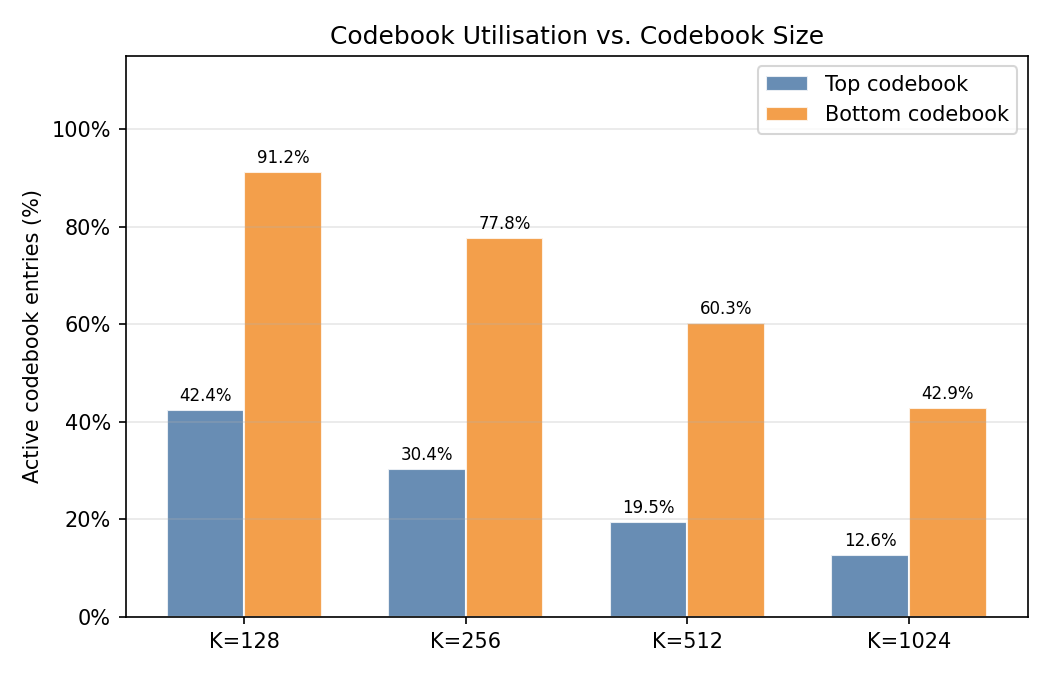
\includegraphics[width=\linewidth]{figures/fig1_utilization.png}
  \caption{Codebook utilisation: fraction of entries active per clip.}
  \label{fig:util}
\end{subfigure}
\hfill
\begin{subfigure}[t]{0.48\linewidth}
  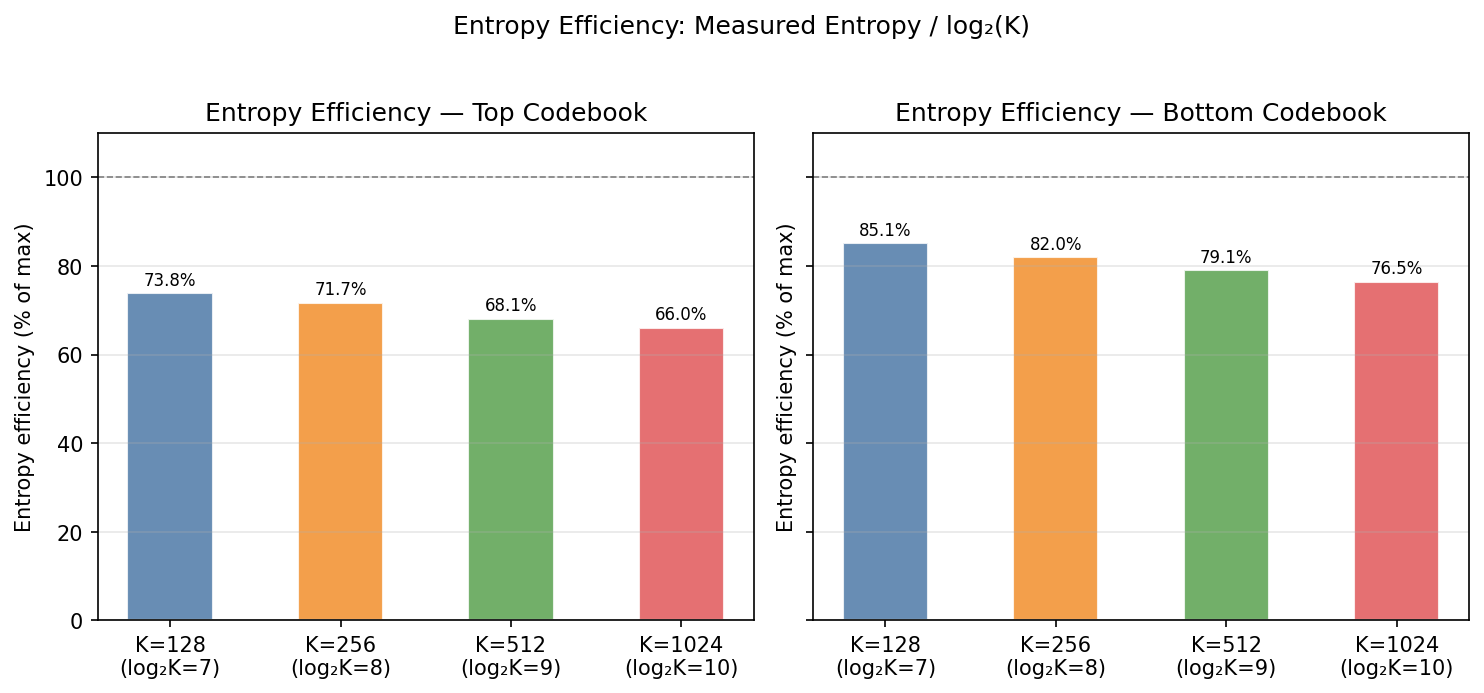
\includegraphics[width=\linewidth]{figures/fig2_entropy_efficiency.png}
  \caption{Entropy efficiency $H(z)/\log_2 K$: how close to the information ceiling.}
  \label{fig:enteff}
\end{subfigure}

\vspace{0.5em}
\begin{subfigure}[t]{0.48\linewidth}
  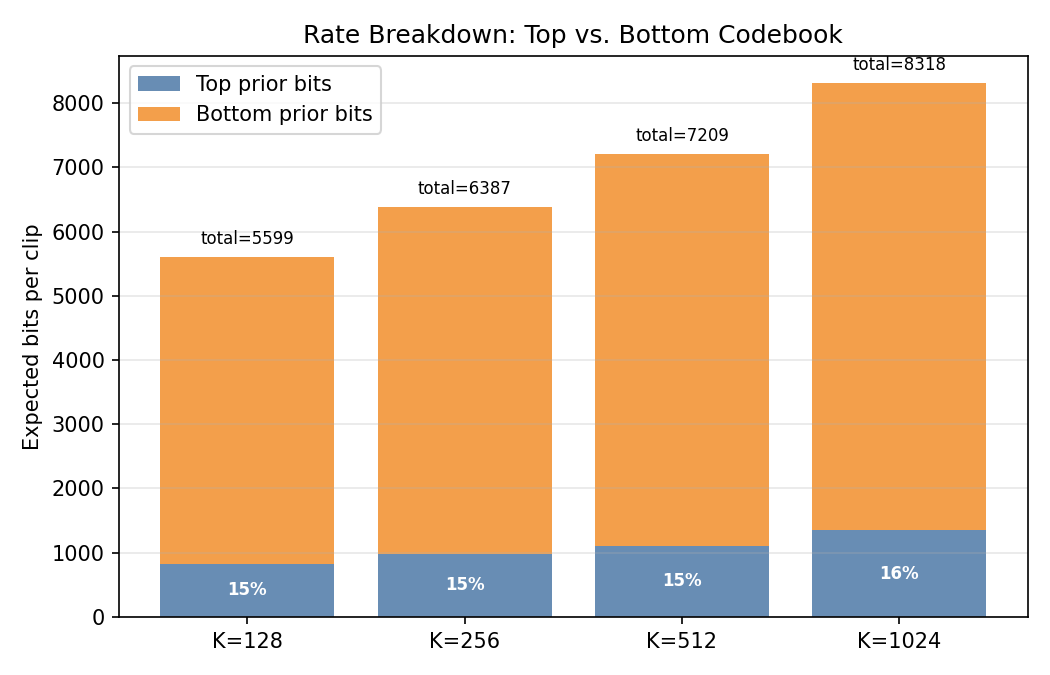
\includegraphics[width=\linewidth]{figures/fig3_rate_breakdown.png}
  \caption{Rate decomposition: expected bits from top vs.\ bottom prior.}
  \label{fig:ratebreak}
\end{subfigure}
\hfill
\begin{subfigure}[t]{0.48\linewidth}
  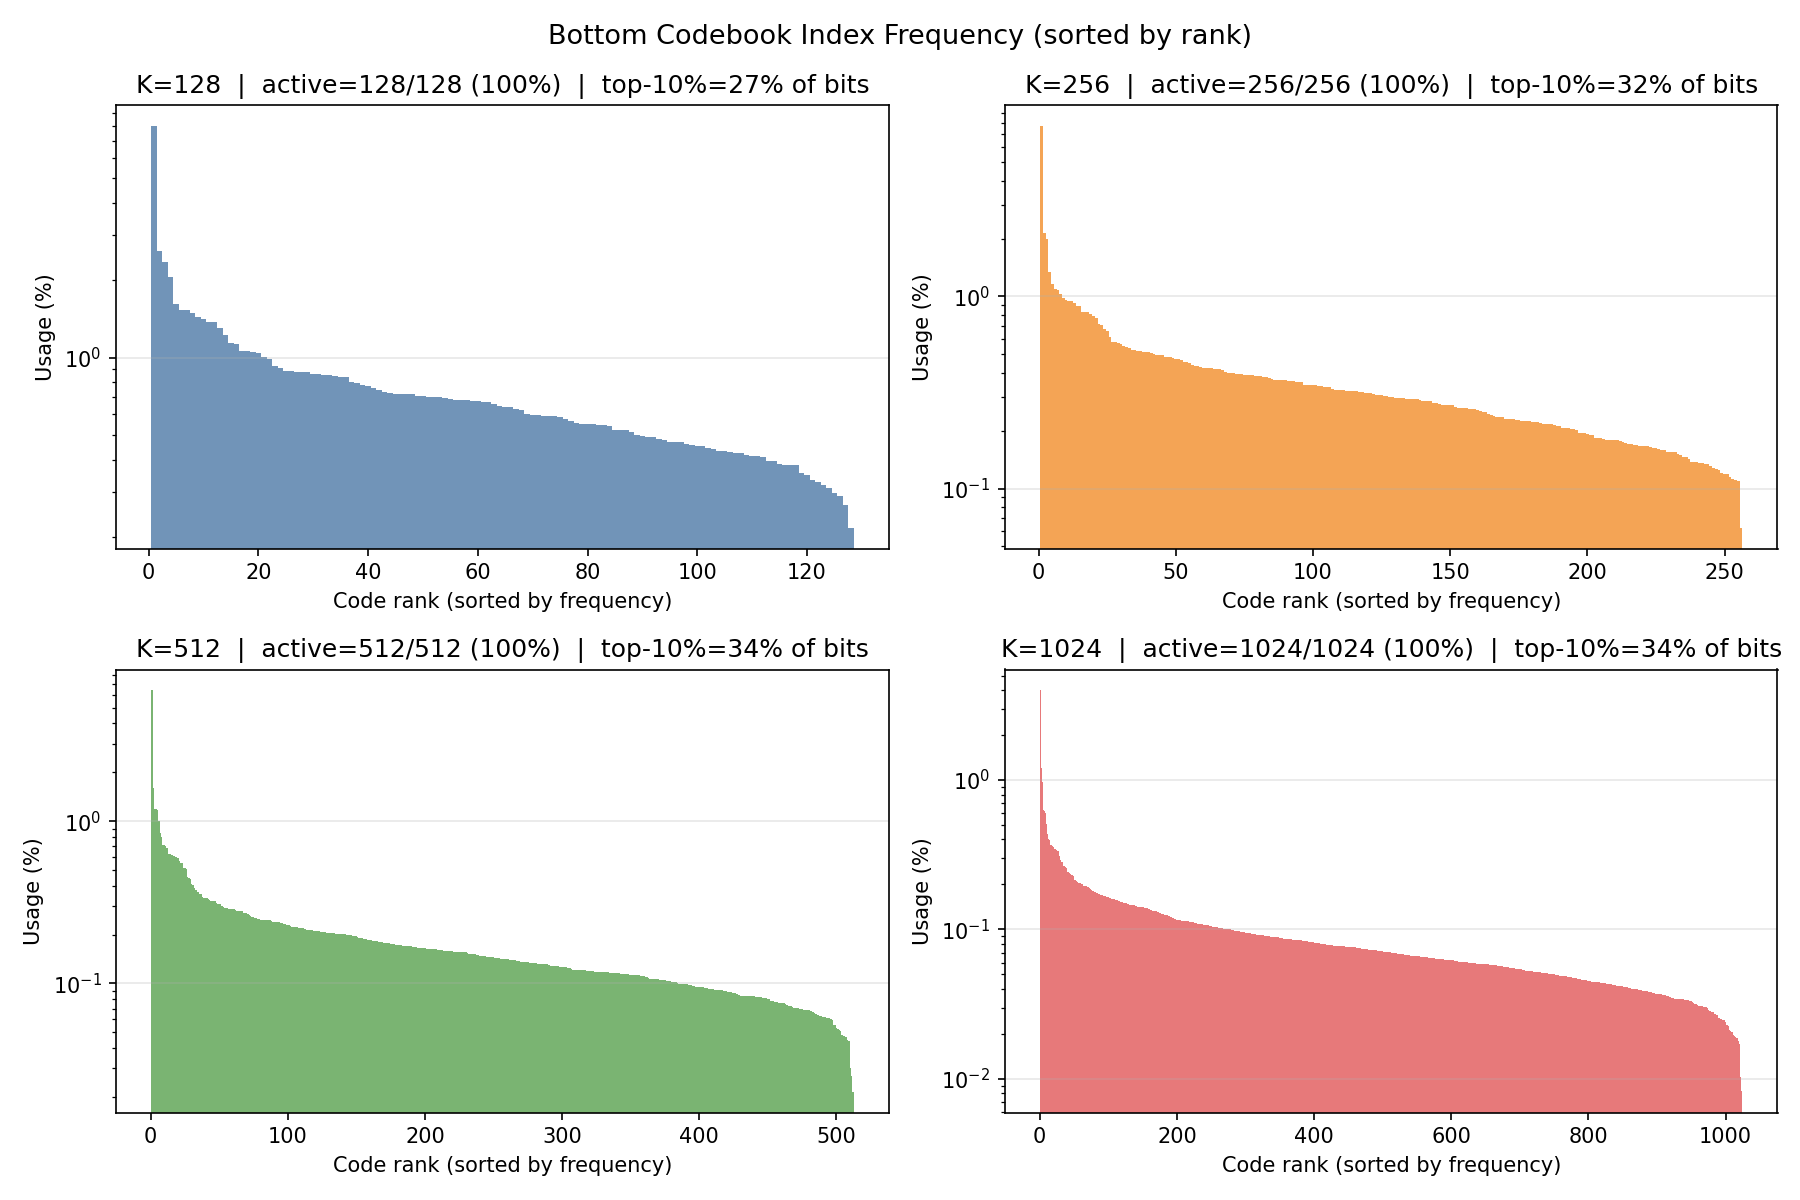
\includegraphics[width=\linewidth]{figures/fig4_index_histogram.png}
  \caption{Index frequency histogram, bottom codebook (log scale).}
  \label{fig:histogram}
\end{subfigure}
\caption{%
  Codebook analysis across $K \in \{128, 256, 512, 1024\}$.
  These four views together characterise how the discrete channel is being used
  and how much compression headroom the priors are exploiting.
}
\label{fig:codebook}
\end{figure}

\paragraph{Utilisation: EMA prevents collapse.}
Figure~\ref{fig:util} shows codebook utilisation (active entries as a
percentage of $K$).
The bottom codebook maintains near-complete utilisation across all $K$ values,
confirming that EMA with dead-code restart successfully prevents collapse.
The top codebook at $K{=}1024$ shows lower utilisation ($\sim\!57\%$),
which is structurally expected: the top grid contains only
$T''\!\times\!H''\!\times\!W'' = 4\!\times\!8\!\times\!8 = 256$ symbols per clip,
so at most 256 of the 1024 entries can be active in any single clip.
The average utilisation over 500 clips reflects the diversity of content
in UCF101 rather than a training failure.

\paragraph{Entropy efficiency: priors capture structure.}
We define entropy efficiency as $\eta = H(z) / \log_2 K$, where $H(z)$ is the
empirical Shannon entropy of the index distribution over the test set.
$\eta = 1$ corresponds to perfectly uniform code usage (no compression
possible beyond the codebook size); $\eta \to 0$ means the model has collapsed
to a single code.
Bottom codebooks achieve $\eta \approx 0.70$--$0.85$
(Figure~\ref{fig:enteff}): the priors capture 15--30\% of the maximum entropy
as structural redundancy, corresponding directly to the compression achieved
beyond $\log_2 K$ bits/symbol.
This efficiency is consistent across $K$ values, suggesting the encoder
develops representations with similar statistical structure regardless of
vocabulary size.

\paragraph{Rate decomposition: bottom codebook dominates.}
Figure~\ref{fig:ratebreak} shows that the bottom codebook contributes
70--80\% of total expected bits across all $K$ values.
This is explained by the asymmetry in grid size:
$N_b/N_t = (T'\!\times\!H'\!\times\!W')\,/\,(T''\!\times\!H''\!\times\!W'')
= (16\!\times\!16\!\times\!16)\,/\,(8\!\times\!8\!\times\!8) = 8$,
so the bottom grid has $8\times$ as many symbols.
The rate grows monotonically with $K$ as expected from Eq.~\ref{eq:bpp}.

\paragraph{Power-law index frequencies: compression beyond the ceiling.}
Figure~\ref{fig:histogram} plots bottom codebook index frequencies sorted
by rank on a log scale.
The near-linear log-log relationship is indicative of a power-law (Zipfian)
distribution: a small fraction of codewords are used for the majority of
symbols.
This heavy-tailed structure is precisely what makes the autoregressive prior
effective---a uniform distribution would leave no information for the prior
to exploit, and BPP would saturate at $\log_2 K$ bits/symbol.
The fact that all four $K$ values show similarly shaped distributions
suggests that the encoder consistently learns to concentrate code usage,
regardless of vocabulary size.

\paragraph{Embedding geometry: organised expansion with $K$.}
Figure~\ref{fig:pca} shows PCA projections of the bottom codebook embeddings.
At $K{=}128$ the embeddings occupy a compact, roughly isotropic region of the
embedding space, consistent with the encoder output distribution being
well-covered by a small vocabulary.
As $K$ increases, the geometry expands and differentiates: at $K{=}1024$
distinct sub-clusters are visible, suggesting that the larger codebook has
partitioned the encoder manifold into semantically coherent regions.
The variance explained by the first two principal components decreases with
$K$ (higher $K$ requires more dimensions to describe the codebook geometry),
confirming that the embedding space is being used more fully.

\begin{figure}[t]
\centering
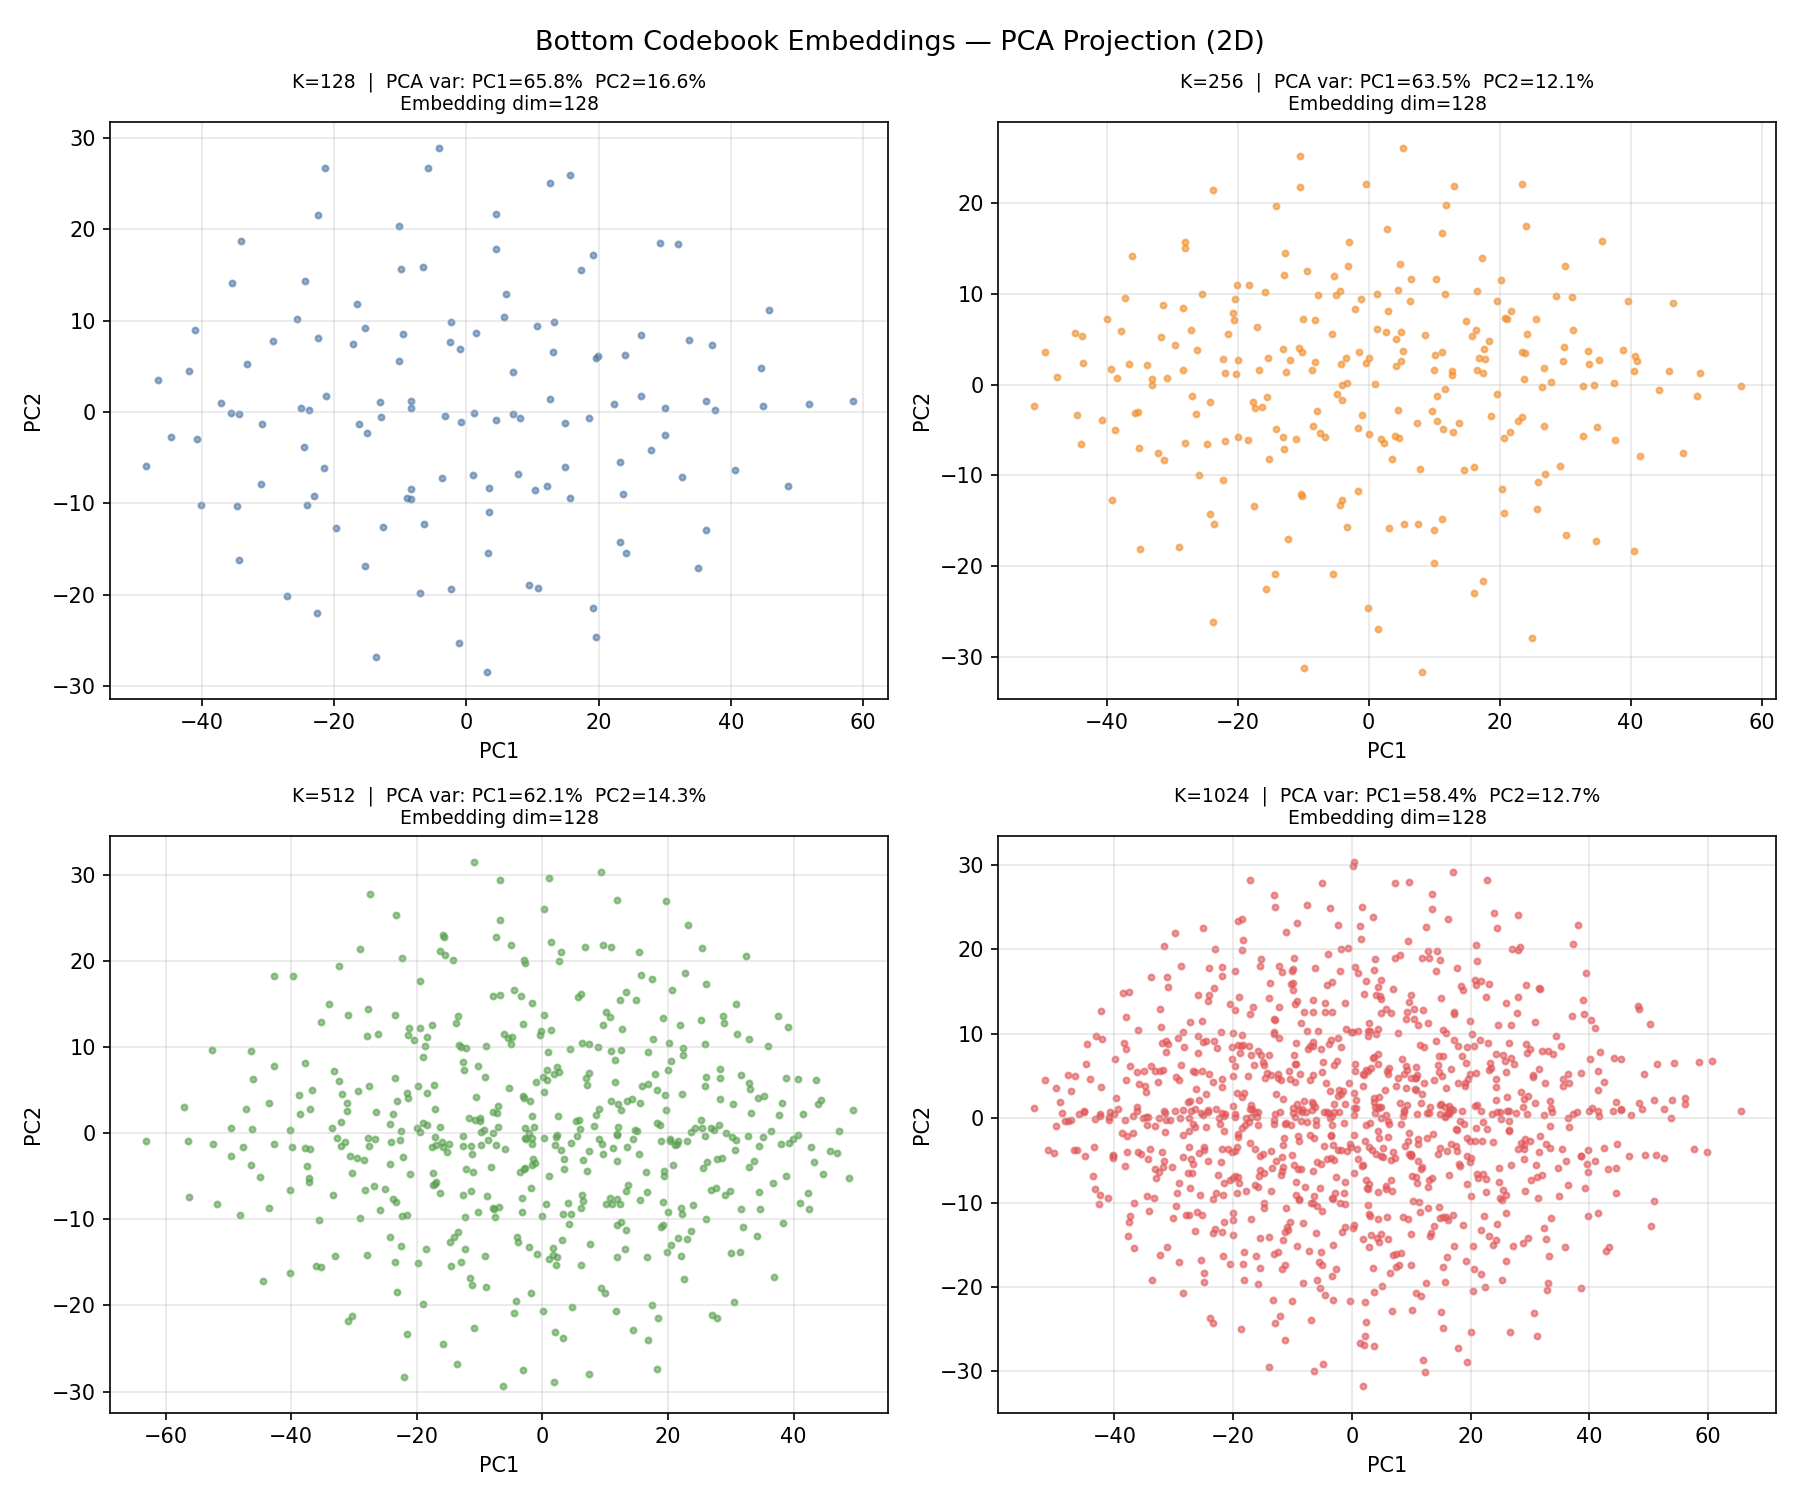
\includegraphics[width=0.85\linewidth]{figures/fig5_embedding_pca.png}
\caption{%
  \textbf{Bottom codebook embeddings: PCA projection to 2D.}
  Each point is a learned codeword; columns correspond to
  $K\in\{128,256,512,1024\}$.
  The embedding geometry expands and differentiates with $K$, consistent
  with finer-grained partitioning of the encoder output manifold.
}
\label{fig:pca}
\end{figure}

% ─────────────────────────────────────────────────────────────────────────────
\section{Discussion}
\label{sec:discussion}

\paragraph{The K-sweep as an information-theoretic rate ladder.}
The central design choice of this work is to use $K$ as the rate-control
parameter rather than a loss weight $\lambda$.
This choice has a clean information-theoretic interpretation.
A VQ codebook with $K$ entries is a discrete channel with capacity
$C = \log_2 K$ bits/symbol.
The actual bitrate is $R = C - \Delta$, where $\Delta \geq 0$ is the
compression achieved by the prior over the uniform distribution.
By varying $K$, we move the channel capacity and hence the achievable
operating range; by training the prior to minimise cross-entropy, we push
$\Delta$ as large as possible at each $K$.
This is fundamentally different from Lagrangian RD, where a single model
is operated at different points on a learned RD curve by changing $\lambda$.
The K-sweep produces a family of models, each optimal for a specific capacity
regime, rather than a single model with variable rate.
Whether one approach dominates the other in practice depends on whether the
cost of training multiple models ($K$-sweep) is acceptable relative to the
flexibility of a single variable-rate model.

\paragraph{Why Lagrangian RD fails for VQ.}
The Lagrangian approach $\mathcal{L} = D + \lambda R$ requires $\partial R /
\partial \theta \neq 0$, where $\theta$ are the encoder parameters.
For continuous-latent models, $R$ is approximated by the log-likelihood under
the entropy model~\cite{balle2018variational,minnen2018joint}, and this
gradient flows back through the encoder.
In VQ-VAE, the $\arg\min$ operation in Eq.~\ref{eq:vq} is non-differentiable,
and the straight-through estimator passes encoder gradients \emph{past} the
quantisation without modifying the code probabilities.
A soft-quantisation approximation (temperature-annealed softmax) does
provide a differentiable rate estimate, but in our experiments the VQ
commitment loss dominated the rate term by $\sim\!600{,}000\times$ in
magnitude, making the rate signal negligible at the gradient level.
This scale mismatch is not easily resolved by re-weighting, since the optimal
weight would vary dramatically across training stages and $K$ values.

\paragraph{Limitations and scope.}
The primary limitation of the K-sweep is \emph{discreteness}: the four
operating points are not easily interpolated, and a target bitrate between
two $K$ values cannot be served without training an additional model.
A natural extension is to condition the encoder on a learnable rate token,
enabling a single model to operate at multiple rates~\cite{mentzer2022vqcompression}.
Second, our evaluation is limited to UCF101 at 64$\times$64;
performance at higher resolutions and on more diverse content (natural
scenes, news, sports) remains to be established.
Third, the autoregressive prior is sequential at inference, adding latency
proportional to $N_t + N_b$ per clip; parallel decoding methods (e.g.\
masked token prediction) could reduce this.
Finally, we compare against H.264 only; a thorough evaluation against H.265,
VVC, and learned codecs (DVC, DCVC) at matched resolution and bitrate would
provide a more complete picture.

\paragraph{Relationship to generative video models.}
Modern video tokenizers (e.g.\ VQGAN-based models for generation) use
architectures similar to ours but are optimised for generation diversity
rather than compression fidelity.
Our work suggests that the compression and generation objectives are not
conflicting: a model optimised for low BPP via learned priors implicitly
learns a compact, structured representation that could serve as a substrate
for conditional generation at ultra-low bitrate.
Exploring this connection is a natural direction for future work.

% ─────────────────────────────────────────────────────────────────────────────
\section{Conclusion}
\label{sec:conclusion}

We have characterised the rate--distortion behaviour of \model{}, a
two-level hierarchical VQ-VAE-2 with 3D autoregressive entropy priors, by
sweeping the codebook size $K$ across four values.
The key insight is that $K$ is not merely a hyperparameter but an
information-theoretic capacity parameter: it sets a hard ceiling on bits per
symbol, and the prior's role is to push actual bitrate as far below that
ceiling as the learned index distribution allows.
EMA-stabilised codebook training with dead-code restart is essential to
realise this capacity across all $K$ values without collapse.

The resulting models operate at 0.043--0.064~bpp---a regime inaccessible to
H.264 at 64$\times$64---and achieve perceptual quality competitive with the
most aggressive H.264 settings at $3.3$--$3.8\times$ lower bitrate.
Codebook analysis reveals well-utilised, power-law distributed discrete
vocabularies with 70--85\% entropy efficiency, confirming that the pipeline
functions as an effective learned entropy coder rather than as a simple
nearest-neighbour lookup.

These results suggest a broader principle: at very low bitrates where
continuous-latent codecs struggle with rate-penalty calibration, discrete
latent models with structured priors offer a principled and interpretable
alternative, with the codebook acting as a controllable information bottleneck.

% ─────────────────────────────────────────────────────────────────────────────
\begin{small}
\bibliography{references}
\end{small}

\end{document}
